\chapter{Hydrogel nuclear pore mimic dataset}~\label{appx:dataset}

This appendix gives the parameters calculated for each hydrogel in the FRAP dataset, organized by FSFG condition.  The predicted values for bound diffusion constant $D_B$ and bound to free diffusion ratio $D_B/D_F$ assume that that the only mechanism of bound diffusion is tethered diffusion, so that $$\frac{D_B}{D_F}  = \frac{L_c \ell_p
    k_\un{off}}{L_c \ell_p k_\un{off} + 3D_F}$$
The parameters used are given in Fig.~\ref{fig:params}.  The $K_D$ values are average values from \cite{hayama18}.  The on-rate $\kon$ is assumed to be diffusion-limited.  Diffusion constants have units of $\mu$m$^2$/s.  Partition coefficients ($\gamma$) and fraction of NTF2 bound ($p_B$) are unitless.

\begin{SCfigure}
\caption[Parameters for predicted bound diffusion.]{Parameters used to predict the bound diffusion constant for NTF2-F in FSFG hydrogels.  Binding data is from \cite{hayama18}.  \\}
\centering
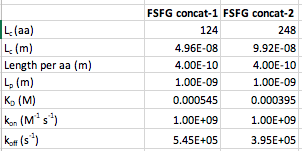
\includegraphics[width=0.4\textwidth]{figs/apps/dataset-params.png}
\label{fig:params}
\end{SCfigure} 

\begin{figure}
\caption[No-Nup hydrogel dataset.]{Measured and calculated values for no-Nup hydrogels.}
\centering
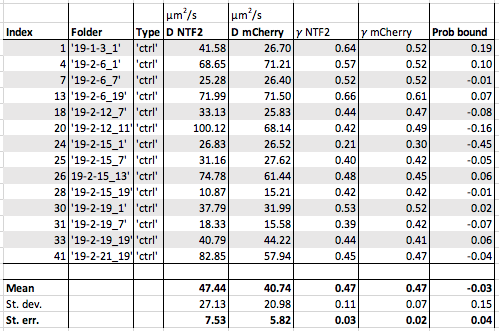
\includegraphics[width=0.7\textwidth]{figs/apps/dataset-ctrl.png}
\label{fig:bound-diffusion}
\end{figure} 

\begin{figure}
\caption[FSFG concat-1 hydrogel dataset.]{Measured and calculated values for FSFG concat-1 hydrogels, nominally containing 10 mg/mL FSFG.}
\centering
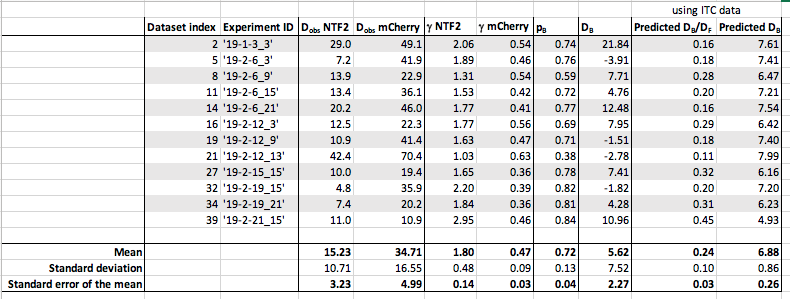
\includegraphics[width=\textwidth]{figs/apps/dataset-cct1.png}
\label{fig:bound-diffusion}
\end{figure} 

\begin{figure}
\caption[FSFG concat-2 hydrogel dataset.]{Measured and calculated values for FSFG concat-2 hydrogels.}
\centering
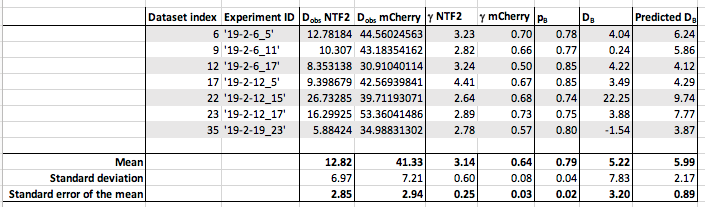
\includegraphics[width=\textwidth]{figs/apps/dataset-cct2.png}
\label{fig:bound-diffusion}
\end{figure} 